\documentclass[12pt,a4paper,twocolumn]{article}

%% ── Packages ──────────────────────────────────────────────────────────
\usepackage[utf8]{inputenc}
\usepackage[T1]{fontenc}
\usepackage{lmodern}
\usepackage{amsmath,amssymb,amsthm}
\usepackage{mathtools}
\usepackage{graphicx}
\usepackage{tikz}
\usetikzlibrary{arrows.meta,positioning,calc,decorations.pathreplacing,shapes.geometric,backgrounds,fit}
\usepackage{pgfplots}
\pgfplotsset{compat=1.18}
\usepackage{booktabs}
\usepackage{multirow}
\usepackage{caption}
\usepackage{subcaption}
\usepackage[hidelinks]{hyperref}
\usepackage{cleveref}
\usepackage{natbib}
\bibliographystyle{plainnat}
\usepackage[margin=2cm]{geometry}
\usepackage{enumitem}
\usepackage{xcolor}

%% ── Theorem environments ──────────────────────────────────────────────
\newtheorem{theorem}{Theorem}[section]
\newtheorem{proposition}[theorem]{Proposition}
\newtheorem{lemma}[theorem]{Lemma}
\newtheorem{corollary}[theorem]{Corollary}
\newtheorem{definition}{Definition}[section]
\newtheorem{remark}{Remark}[section]
\newtheorem{example}{Example}[section]

%% ── Custom commands ───────────────────────────────────────────────────
\newcommand{\N}{\mathcal{N}}
\newcommand{\D}{\mathcal{D}}
\newcommand{\CC}{\mathcal{C}}
\newcommand{\R}{\mathbb{R}}
\newcommand{\Sust}{\mathrm{S}}
\newcommand{\Ebase}{E_{\mathrm{base}}}
\newcommand{\argmin}{\operatorname{arg\,min}}
\newcommand{\tholon}{\mathfrak{T}}

%% ── Colors for diagrams ──────────────────────────────────────────────
\definecolor{Ncolor}{HTML}{1A6EFA}
\definecolor{Dcolor}{HTML}{F85149}
\definecolor{Ccolor}{HTML}{3FB950}
\definecolor{stdcolor}{HTML}{4FA3FF}
\definecolor{thocolor}{HTML}{F0C040}

%% ── Title ─────────────────────────────────────────────────────────────
\title{%
  \textbf{Beyond Nash Equilibrium: Tholonic Triadic Dynamics\\
  as a Sustainability-Oriented Alternative to Classical Game Theory\\
  in Supply Chain and Value Chain Systems}%
}

\author{%
  \textsc{Working Paper}\\[4pt]
  {\normalsize Supply Chain Intelligence Project}\\
  {\small\texttt{draft---v1.0 / February 2026}}%
}

\date{}

%% ══════════════════════════════════════════════════════════════════════
\begin{document}
\maketitle

%% ── Abstract ──────────────────────────────────────────────────────────
\begin{abstract}
\noindent
Classical game theory, grounded in Nash equilibrium and rational-actor assumptions, has dominated the formal analysis of strategic interaction in economics, supply chain management, and mechanism design for over seven decades.
Yet its core predictions---particularly the tragedy of the commons and the prisoner's dilemma---remain descriptive of failure rather than prescriptive of sustainability.
This paper introduces the \emph{tholonic model}, a triadic framework in which every system is decomposed into three archetypal forces: \emph{Definition} ($\D$, constraint/structure), \emph{Contribution} ($\CC$, integration/flow), and \emph{Negotiation} ($\N$, emergent equilibrium).
We show formally that the tholonic sustainability condition---$\D \approx \CC$, minimizing maintenance energy---generalises the Nash equilibrium concept while embedding resource-awareness and hierarchical self-similarity absent from standard game-theoretic models.
Through analytical comparison, agent-based simulation, and application to multi-phase supply chain and value chain networks, we demonstrate that tholonic dynamics produce cooperative equilibria that resist commons collapse, predict phase-specific bottlenecks invisible to aggregate game-theoretic analysis, and provide a unified optimisation framework spanning physical logistics, economic value creation, and systemic resilience.
We discuss implications for economics, operations research, systems theory, and sustainability science.

\medskip
\noindent\textbf{Keywords:} game theory, tholonic model, N-D-C dynamics, supply chain optimization, value chain analysis, sustainability, complex adaptive systems, cooperative equilibrium, tragedy of the commons, systems theory
\end{abstract}

%% ══════════════════════════════════════════════════════════════════════
\section{Introduction}
\label{sec:intro}

The analytical toolkit available to economists, operations researchers, and supply chain practitioners for modelling strategic interaction has been overwhelmingly shaped by non-cooperative game theory \citep{vonNeumann1944,Nash1950,Nash1951}.
The central solution concept---Nash equilibrium---identifies states from which no individual agent can unilaterally improve its payoff.
While mathematically elegant, Nash equilibrium is agnostic to the sustainability of the state it describes: a tragedy-of-the-commons outcome, in which a shared resource is depleted to the detriment of all participants, is as valid a Nash equilibrium as a Pareto-optimal allocation \citep{Hardin1968,Ostrom1990}.

This limitation is not merely academic.
In commodity supply chains---gold, agricultural products, rare earths---the physical system imposes constraints that classical game theory treats as exogenous parameters rather than endogenous dynamics.
A gold refinery operating at 99.99\% purity standards (a \emph{definitional} constraint) must simultaneously maintain flexible supplier networks (a \emph{contributive} integration); the emergent operational state is neither purely competitive nor purely cooperative, but a dynamic negotiation between structure and flow.
Standard game-theoretic models flatten this triadic structure into a payoff matrix, losing the information that determines long-term viability.

This paper presents the \textbf{tholonic model} as an alternative and extension.
The tholonic framework decomposes every system---from an individual transaction to an entire industry---into three interacting forces:

\begin{itemize}[nosep]
  \item $\D$ (\textbf{Definition}): constraint, boundary, specification, internal coherence;
  \item $\CC$ (\textbf{Contribution}): integration, connection, flow, external exchange;
  \item $\N$ (\textbf{Negotiation}): the emergent equilibrium that arises from $\D$--$\CC$ interaction.
\end{itemize}

The tholonic model is not a repudiation of game theory; it is a \emph{re-grounding} of strategic interaction within a physically and thermodynamically informed ontology.
Where game theory asks ``What is the rational strategy?'', the tholonic model asks ``What configuration is sustainable?''---and it provides a formal criterion: systems minimise maintenance energy when $\D \approx \CC$, a condition we term \emph{tholonic balance}.

The remainder of this paper is organised as follows.
\Cref{sec:philosophy} situates the tholonic model within systems theory and philosophy of science.
\Cref{sec:gametheory} reviews classical game theory and identifies its structural limitations.
\Cref{sec:tholonic} formalises the tholonic framework mathematically.
\Cref{sec:comparison} provides a rigorous side-by-side comparison.
\Cref{sec:supplychain} applies both frameworks to multi-phase supply chain modelling.
\Cref{sec:valuechain} extends the analysis to value chains and economic surplus.
\Cref{sec:simulation} presents agent-based simulation results.
\Cref{sec:discussion} discusses implications and limitations.
\Cref{sec:conclusion} concludes.

%% ══════════════════════════════════════════════════════════════════════
\section{Philosophical and Systems-Theoretic Foundations}
\label{sec:philosophy}

\subsection{From Atomism to Triadic Ontology}

Classical game theory inherits the atomistic ontology of neoclassical economics: agents are fundamental, preferences are given, and interaction is mediated through payoff functions defined over discrete strategy sets \citep{Mas-Colell1995}.
This framework is profoundly \emph{dualistic}: it recognises only two categories---agents and their environment---and models interaction as bilateral exchange.

The tholonic model draws instead from a \emph{triadic} ontological tradition with deep roots in process philosophy \citep{Whitehead1929}, general systems theory \citep{vonBertalanffy1968}, and dissipative structures \citep{Prigogine1984}.
In the Peircean semiotic tradition, every sign relation requires three irreducible components: sign, object, and interpretant \citep{Peirce1931}.
Analogously, every tholonic system requires three irreducible forces: structure ($\D$), flow ($\CC$), and the emergent state ($\N$) that mediates between them.

This triadic structure is not an arbitrary choice.
It reflects a fundamental observation about complex systems: \emph{no system can be understood through its constraints alone or its connections alone}; it is the interaction between boundary-making and boundary-crossing that generates observable reality.
This insight is shared by autopoietic theory \citep{Maturana1980}, where systems maintain identity (analogous to $\D$) through interaction with their environment (analogous to $\CC$), producing self-referential organisation (analogous to $\N$).

\subsection{Thermodynamic Grounding}

The tholonic model embeds thermodynamic principles that game theory lacks.
In classical game theory, the ``cost'' of a strategy is defined purely in terms of opportunity cost within the payoff structure; there is no concept of the \emph{energy required to maintain a strategic position}.

The tholonic framework introduces \emph{maintenance energy}:

\begin{equation}
\label{eq:maintenance}
E_{\mathrm{maint}} = |\D - \CC|^\alpha + \Ebase
\end{equation}

where $\alpha \geq 2$ is a system-specific exponent and $\Ebase > 0$ is the irreducible baseline energy cost of existence.
This formulation has direct analogues in Landauer's principle \citep{Landauer1961}---the minimum energy cost of information processing---and in the thermodynamics of self-organisation \citep{England2013}, where dissipative structures must continuously expend energy to maintain themselves far from equilibrium.

\emph{Sustainability} is then defined as the inverse of maintenance energy:

\begin{equation}
\label{eq:sustainability}
\Sust(\D, \CC) = \frac{1}{|\D - \CC|^\alpha + \Ebase}
\end{equation}

This provides a principled, physically grounded objective function that is entirely absent from classical game theory.

\subsection{Self-Similarity and Hierarchical Composition}

A distinguishing feature of the tholonic model is its \emph{fractal architecture}.
Each tholon ($\tholon$) at scale $i$ decomposes into a complete $\N$-$\D$-$\CC$ structure at scale $i-1$:

\begin{equation}
\label{eq:recursion}
\tholon_i = \N_i\bigl(\D_i(\tholon_{i-1}^{(D)}),\; \CC_i(\tholon_{i-1}^{(C)})\bigr)
\end{equation}

This recursive composition is isomorphic to the renormalisation group in statistical physics \citep{Wilson1971}, where macroscopic behaviour emerges from iterated application of the same dynamical laws across scales.

Game theory possesses no native mechanism for hierarchical self-similarity.
While extensive-form games can represent sequential decisions and subgame perfection \citep{Selten1965} provides refinement within hierarchies, the underlying strategic structure does not repeat across scales---a payoff matrix at the firm level bears no structural resemblance to a payoff matrix at the industry level.
The tholonic model's self-similarity, by contrast, ensures that insights gained at any scale transfer to all others, a property of enormous practical value in supply chain analysis where micro-transactions, meso-relationships, and macro-networks must be analysed coherently.

%% ══════════════════════════════════════════════════════════════════════
\section{Classical Game Theory: Foundations and Limitations}
\label{sec:gametheory}

\subsection{Nash Equilibrium and Its Discontents}

A \emph{normal-form game} $\Gamma = (I, \{S_i\}_{i \in I}, \{u_i\}_{i \in I})$ consists of a finite set of players $I$, strategy sets $S_i$, and payoff functions $u_i: \prod_j S_j \to \R$.
A strategy profile $s^* = (s_1^*, \ldots, s_n^*)$ is a \emph{Nash equilibrium} if:

\begin{equation}
\label{eq:nash}
u_i(s_i^*, s_{-i}^*) \geq u_i(s_i, s_{-i}^*) \quad \forall i \in I,\; \forall s_i \in S_i
\end{equation}

The Nash equilibrium concept is subject to well-documented limitations:

\begin{enumerate}[nosep,label=(\roman*)]
  \item \textbf{Multiplicity:} Games typically admit multiple Nash equilibria with no principled selection criterion \citep{Harsanyi1988}.
  \item \textbf{Sustainability blindness:} The equilibrium concept is \emph{static}; it identifies fixed points but says nothing about whether they can be maintained over time under resource constraints.
  \item \textbf{Commons collapse:} In public goods games, the unique Nash equilibrium is universal defection---the tragedy of the commons \citep{Hardin1968}---despite its collective irrationality.
  \item \textbf{Exogenous structure:} The game's structure (players, strategies, payoffs) is given \emph{a priori}; there is no mechanism for the game itself to evolve.
  \item \textbf{No resource dynamics:} Payoff functions are fixed and do not depend on accumulated resource levels or system health.
\end{enumerate}

\subsection{Extensions and Their Insufficiency}

Mechanism design \citep{Myerson1981} and evolutionary game theory \citep{MaynardSmith1982} partially address these limitations.
Mechanism design constructs incentive-compatible institutions but requires a principal with complete information about the game's structure---a condition rarely met in supply chains.
Evolutionary game theory introduces population dynamics and selection but operates on \emph{strategies}, not on the \emph{structural configuration} of the system itself.

Repeated games with discounting \citep{Fudenberg1991} can sustain cooperation through folk-theorem arguments, but the resulting equilibria are sustained by \emph{threat} (reversion to punishment strategies), not by \emph{structural balance}.
The cooperation is fragile: it depends on precise beliefs about discount factors and monitoring capacity.

Ostrom's institutional analysis \citep{Ostrom1990,Ostrom2005} demonstrates empirically that communities develop governance structures to avoid commons tragedy, but this work lacks a formal mathematical framework connecting institutional design to system sustainability.

The tholonic model, as we show below, provides such a framework.

%% ══════════════════════════════════════════════════════════════════════
\section{The Tholonic Framework: Mathematical Formalisation}
\label{sec:tholonic}

\subsection{Definitions}

\begin{definition}[Tholon]
\label{def:tholon}
A \emph{tholon} is a triple $\tholon = (\D, \CC, \N)$ where:
\begin{itemize}[nosep]
  \item $\D \in \R^n_+$ is the \emph{Definition vector} (constraint intensities);
  \item $\CC \in \R^m_+$ is the \emph{Contribution vector} (integration intensities);
  \item $\N: \R^n_+ \times \R^m_+ \to \R_+$ is the \emph{Negotiation function} producing the emergent state.
\end{itemize}
\end{definition}

\begin{definition}[Aggregate Magnitudes]
\label{def:aggregates}
Given weight vectors $\mathbf{w}^D \in \R^n_+$ and $\mathbf{w}^C \in \R^m_+$:
\begin{align}
D &\coloneqq \sum_{i=1}^n w_i^D \cdot d_i = \mathbf{w}^D \cdot \D \\
C &\coloneqq \sum_{j=1}^m w_j^C \cdot c_j = \mathbf{w}^C \cdot \CC
\end{align}
\end{definition}

\subsection{The Negotiation Operator}

The central equation of the tholonic model defines the emergent $\N$-state as the energy-minimising configuration:

\begin{equation}
\label{eq:nstate}
\N^* = \argmin_{\N} \bigl[ E_D + E_C + E_{\mathrm{int}}(\D, \CC, \N) \bigr]
\end{equation}

Under the specific functional form used in simulation:

\begin{equation}
\label{eq:nvalue}
N = \sqrt{D \cdot C} \cdot \beta(D, C)
\end{equation}

where the \emph{balance factor} $\beta$ is:

\begin{equation}
\label{eq:balance}
\beta(D, C) = \exp\!\left(-\frac{2\,|D - C|}{\max(D, C)}\right)
\end{equation}

\begin{proposition}[Balance Maximises N]
\label{prop:balance}
For fixed $D + C = K$ (constant total resources), $N$ is maximised when $D = C = K/2$.
\end{proposition}

\begin{proof}
With $D + C = K$ and $D = K/2 + \delta$, $C = K/2 - \delta$:
\[
N(\delta) = \sqrt{\tfrac{K^2}{4} - \delta^2}\; \exp\!\Bigl({-}\tfrac{4|\delta|}{K/2 + |\delta|}\Bigr)
\]
The geometric mean $\sqrt{(K/2)^2 - \delta^2}$ is maximised at $\delta = 0$ (AM-GM inequality), and $\beta$ is maximised at $\delta = 0$ (exponent is zero).
Since both factors are maximised at $\delta = 0$, their product is maximised at $D = C = K/2$.
\end{proof}

\subsection{Sustainability and Energy Landscape}

\begin{definition}[Tholonic Sustainability]
\label{def:sustainability}
The sustainability of a tholon is:
\begin{equation}
\label{eq:sust}
\Sust(D, C) = \frac{100}{|D - C|^2 + \Ebase}
\end{equation}
where $\Ebase > 0$ is the baseline energy cost.
\end{definition}

The energy landscape over $(D, C)$-space defines a potential surface:

\begin{multline}
\label{eq:potential}
U(D, C) = (D {-} C)^2 + \Ebase \\
  + \lambda_D {\textstyle\sum_i} \phi_D(d_i) + \lambda_C {\textstyle\sum_j} \phi_C(c_j)
\end{multline}

where $\phi_D$ and $\phi_C$ are per-parameter cost functions (quadratic for $\D$, superlinear for $\CC$ due to coordination overhead).

\subsection{Stability Analysis}

The dynamic evolution of a tholon is governed by:

\begin{equation}
\label{eq:dynamics}
\frac{d}{dt}\begin{pmatrix} D \\ C \\ N \end{pmatrix} = \begin{pmatrix}
\alpha_D(D^* - D) - \beta_D \cdot D \cdot P \\
\alpha_C(C^* - C) - \beta_C \cdot C \cdot P \\
k_1 DC - k_2 N - k_3 N |D - C|
\end{pmatrix}
\end{equation}

where $D^*, C^*$ are targets, $P$ is cost pressure, and $k_1, k_2, k_3$ are rate constants.

\begin{proposition}[Stability at Balance]
\label{prop:stability}
The equilibrium point $D^* = C^*$ is a stable node: all eigenvalues of the Jacobian $\mathbf{J}$ evaluated at $(D^*, C^*, N^*)$ with $D^* = C^*$ have strictly negative real parts.
\end{proposition}

\begin{proof}[Proof sketch]
At $D = C$, the $|D-C|$ terms vanish and the cross-coupling terms in the Jacobian reduce to symmetric form.
The diagonal elements $\partial F_D/\partial D = -\alpha_D - \beta_D P$ and $\partial F_C/\partial C = -\alpha_C - \beta_C P$ are strictly negative for positive parameters.
The off-diagonal coupling through $N$ is bounded, and the Routh--Hurwitz conditions are satisfied for physically meaningful parameter ranges.
\end{proof}

%% ══════════════════════════════════════════════════════════════════════
\section{Formal Comparison: Game Theory vs.\ Tholonic Dynamics}
\label{sec:comparison}

\subsection{Structural Correspondence}

We establish a mapping between the two frameworks:

\begin{table}[ht]
\centering
\scriptsize
\caption{Structural correspondence between game-theoretic and tholonic concepts.}
\label{tab:correspondence}
\begin{tabular}{@{}p{1.5cm}p{2.5cm}p{2.8cm}@{}}
\toprule
\textbf{Concept} & \textbf{Game Theory} & \textbf{Tholonic Model} \\
\midrule
Agents & Players $I$ & Tholons $\tholon$ \\
Choices & Strategy set $S_i$ & $\D$--$\CC$ config. \\
Outcome & Payoff $u_i(s)$ & $\N$-state $N(D,C)$ \\
Equilib. & Nash: no unilateral deviation gain & Balance: $D \approx C$ minimises energy \\
Optimal. & Pareto efficiency & Sustainability $\Sust$ \\
Dynamics & Replicator eq. & \Cref{eq:dynamics} \\
Hierarchy & Subgames & Thologram recursion \\
Resource & Exogenous & Endogenous $R(t)$ \\
\bottomrule
\end{tabular}
\end{table}

\subsection{The Public Goods Game: A Comparative Analysis}

Consider $n$ agents sharing a common resource $R \in [0, 1]$.
Each round, agent $i$ chooses to cooperate ($a_i = 1$, cost $c$) or defect ($a_i = 0$).
The public good payoff is $g = b \cdot R \cdot \sum_i a_i / n$, where $b$ is the benefit multiplier.

\subsubsection{Standard Game-Theoretic Analysis}

Each agent updates cooperation probability $p_i$ via reinforcement:

\begin{equation}
\label{eq:standard_update}
p_i \leftarrow p_i + \eta \cdot \begin{cases} +1 & \text{if } a_i = 1 \text{ and } \pi_i > 0 \\ -1 & \text{if } a_i = 1 \text{ and } \pi_i \leq 0 \end{cases}
\end{equation}

where $\pi_i = g - a_i \cdot c$ and $\eta$ is the learning rate.
The resource evolves as:

\begin{multline}
R_{t+1} = \mathrm{clamp}\!\bigl(R_t + r_{\mathrm{reg}} \cdot \bar{a} \\
  - r_{\mathrm{dec}} \cdot (1 - \bar{a})\bigr)
\end{multline}

where $\bar{a} = \sum_i a_i / n$ is the cooperation fraction.

Under standard analysis, when $c > b \cdot R / n$ (which holds for moderate $n$), the individually rational strategy is defection.
The unique Nash equilibrium is $p_i \to 0 \;\forall i$, leading to $R \to 0$: commons collapse.

\subsubsection{Tholonic Analysis}

The tholonic model augments each agent's update with a \emph{sustainability signal}:

\begin{equation}
\label{eq:tholonic_update}
\pi_i^{\mathrm{tho}} = \pi_i + \lambda \cdot (1 - R) \cdot (2a_i - 1)
\end{equation}

where $\lambda \geq 0$ is the tholonic coupling parameter.
When $R$ is low (resource threatened), cooperators receive a bonus $+\lambda(1-R)$ and defectors receive a penalty $-\lambda(1-R)$.
This corresponds to each agent receiving information about the $\D$--$\CC$ balance of the parent system:

\begin{itemize}[nosep]
  \item Low $R$ indicates $\D$-dominance (resource depletion $=$ over-constraint);
  \item The $\lambda$ signal encodes the tholonic principle that contribution to the parent context is essential for the child's viability.
\end{itemize}

\begin{theorem}[Tholonic Cooperation Sustainability]
\label{thm:cooperation}
For $\lambda > c / (1 - R_{\min})$ where $R_{\min}$ is the minimum stable resource level, the tholonic public goods game admits a stable cooperative equilibrium with $p_i > 0.5$ for all $i$ and $R > R_{\min}$.
\end{theorem}

\begin{proof}[Proof sketch]
At the cooperative equilibrium, $\sum a_i / n \approx \bar{p}$ and $R$ stabilises at $R^* = r_{\mathrm{regen}} \bar{p} / (r_{\mathrm{regen}} \bar{p} + r_{\mathrm{decay}}(1-\bar{p}))$.
The tholonic payoff for a cooperator is $\pi_{\mathrm{coop}} = g - c + \lambda(1-R^*)$.
For this to be positive (sustaining cooperation), we need $\lambda(1-R^*) > c - g$, which holds when $\lambda$ exceeds $c/(1-R_{\min})$.
Stability follows from the contraction mapping property: higher cooperation $\to$ higher $R$ $\to$ lower sustainability signal $\to$ equilibrium (negative feedback).
\end{proof}

\subsection{Comparative Properties}

\begin{table}[ht]
\centering
\scriptsize
\caption{Comparative properties in the public goods setting.}
\label{tab:comparison}
\begin{tabular}{@{}p{1.8cm}p{2.4cm}p{2.6cm}@{}}
\toprule
\textbf{Property} & \textbf{Game Theory} & \textbf{Tholonic Model} \\
\midrule
Equilibrium & Universal defection & Cooperative for $\lambda > \lambda^*$ \\
Resource & Collapse ($R \to 0$) & Sustained ($R > R_{\min}$) \\
Information & Payoff only & Payoff + system state \\
Cooperation & Threat-based & Structural balance \\
Scalability & Fixed player set & Hierarchical recursion \\
Resolution & Aggregate & Per-phase $\D$-$\CC$ \\
Objective & Individual payoff & System sustainability \\
\bottomrule
\end{tabular}
\end{table}

The crucial distinction is \emph{ontological}: game theory treats the resource as a passive backdrop; the tholonic model treats the resource as a constitutive element of the system whose health feeds back into agent decision-making.

%% ══════════════════════════════════════════════════════════════════════
\section{Application to Supply Chain Economics}
\label{sec:supplychain}

\subsection{Supply Chains as Tholonic Structures}

A supply chain is a sequence of transformations that convert raw inputs into finished goods, each characterised by physical state changes, custody transfers, and measurable throughput.
We model a supply chain as an ordered set of tholons $\{\tholon_0, \tholon_1, \ldots, \tholon_K\}$ with inter-phase coupling:

\begin{definition}[Supply Chain Thologram]
A \emph{supply chain thologram} is a directed graph $G = (V, E)$ where:
\begin{itemize}[nosep]
  \item $V = \{\tholon_k\}_{k=0}^K$ are phase-tholons, each with $(D_k, C_k, N_k)$;
  \item $E \subseteq V \times V$ are coupling edges with weights $(\gamma_{DC}, \gamma_{CD})$ governing constraint propagation.
\end{itemize}
\end{definition}

\subsubsection{Mapping Physical Supply Chain Elements to $\D$-$\CC$}

The tholonic decomposition maps naturally onto supply chain fundamentals:

\textbf{Definition ($\D$) components} correspond to the structural and regulatory constraints at each phase: product specifications, process protocols, quality standards, capacity limits, regulatory compliance, contractual obligations, and inventory policies.

\textbf{Contribution ($\CC$) components} correspond to the integrative and relational capacities: supplier network breadth, distribution channel diversity, information system connectivity, logistics flexibility, financial instrument access, stakeholder collaboration depth, and technology adoption rate.

Each component is scored on a $[0, 100]$ intensity scale and aggregated:
\begin{equation}
D_k = \sum_{i=1}^{n_k} w_i^{(k)} d_i^{(k)}, \qquad C_k = \sum_{j=1}^{m_k} v_j^{(k)} c_j^{(k)}
\end{equation}

\subsection{Constraint Propagation and Bottleneck Formation}

A key advantage of the tholonic framework over game-theoretic supply chain models \citep{Cachon2003,Nagarajan2008} is its ability to model \emph{constraint propagation}:

\begin{equation}
\label{eq:propagation}
\Delta D_{k+1} = \gamma_{DC}^{(k,k+1)} \cdot \frac{[\max(0,D_k{-}C_k)]^2}{D_k}
\end{equation}

When phase $k$ is $\D$-dominant (over-constrained), it propagates definitional pressure downstream, forcing phase $k+1$ to tighten its own constraints.
Symmetrically, $\CC$-dominance propagates integration demands upstream.

\begin{definition}[Bottleneck]
Phase $k$ is a \emph{bottleneck} if:
\begin{equation}
\frac{|D_k - C_k|}{\max(D_k, C_k)} > \theta_{\mathrm{crit}}
\end{equation}
where $\theta_{\mathrm{crit}} \approx 0.3$ is the critical imbalance threshold.
\end{definition}

In game-theoretic supply chain models, bottlenecks appear only through the lens of capacity constraints or contract structure; the tholonic model reveals bottlenecks as $\D$-$\CC$ imbalances, which may arise from \emph{relational} deficits (insufficient supplier diversity, poor information integration) rather than physical capacity limits.

\subsection{Economic Efficiency and Deadweight Loss}

The tholonic framework provides a novel decomposition of economic inefficiency.
Define the \emph{theoretical maximum} output of phase $k$ as $N_k^{\max} = \sqrt{D_k \cdot C_k}$ (achieved at perfect balance).
The \emph{actual} output is $N_k = N_k^{\max} \cdot \beta(D_k, C_k)$.
The \emph{tholonic deadweight loss} is:

\begin{equation}
\label{eq:dwl}
\mathrm{DWL}_k = N_k^{\max} - N_k = \sqrt{D_k C_k}\bigl(1 - \beta(D_k, C_k)\bigr)
\end{equation}

This maps directly onto the economic concept of allocative inefficiency: resources are being consumed to maintain an imbalanced configuration that a balanced configuration would not require.
Summing across phases:

\begin{equation}
\mathrm{DWL}_{\mathrm{total}} = \sum_{k=0}^{K} \sqrt{D_k C_k}\bigl(1 - \beta_k\bigr)
\end{equation}

This total deadweight loss is \emph{invisible} to standard game-theoretic analysis, which lacks the phase-resolved structure to decompose aggregate inefficiency into its constituent imbalances.

\subsection{Comparative Statics: Gold Supply Chain Example}

Consider a simplified gold supply chain with phases: Extraction ($k=1$), Processing ($k=2$), Refining ($k=4$), and Vaulting ($k=6$).
\Cref{tab:gold_ndc} presents representative $\D$-$\CC$ scores.

\begin{table}[ht]
\centering
\scriptsize
\caption{N-D-C analysis of gold supply chain phases. $\beta$: balance factor.}
\label{tab:gold_ndc}
\begin{tabular}{@{}lrrrrl@{}}
\toprule
\textbf{Phase} & $D$ & $C$ & $\beta$ & $N$ & \textbf{Status} \\
\midrule
Extraction & 270 & 260 & .93 & 246 & Healthy \\
Processing & 400 & 250 & .47 & 149 & $\D$-dom. \\
Refining   & 310 & 290 & .87 & 261 & Good \\
Vaulting   & 420 & 180 & .32 &  88 & Critical \\
\bottomrule
\end{tabular}
\end{table}

The vaulting phase ($k=6$) exhibits severe $\D$-dominance: extremely high security, insurance, and jurisdictional compliance requirements ($D = 420$) combined with limited vault network access, transport inflexibility, and information opacity ($C = 180$).
The balance factor of 0.32 indicates that the phase operates at only 32\% of its theoretical capacity---a finding that game-theoretic models, which lack the $\D$-$\CC$ decomposition, cannot diagnose.

%% ══════════════════════════════════════════════════════════════════════
\section{Value Chain Extension: From Physical Flow to Economic Surplus}
\label{sec:valuechain}

\subsection{Motivation: Why Value Chains Require Separate Treatment}

The tholonic framework respects a strict analytical layering:

\begin{enumerate}[nosep]
  \item \textbf{Supply chain} (physical layer): material flow, custody, physical constraints.
  \item \textbf{Value chain} (economic layer): margin capture, price formation, profit distribution.
  \item \textbf{Financial abstraction} (claims layer): paper claims, leverage, rehypothecation.
\end{enumerate}

This separation is methodologically essential: the supply chain determines \emph{what is physically possible}; the value chain determines \emph{how economic surplus is distributed} across what is possible.
Game-theoretic models of supply chains \citep{Cachon2003} typically conflate these layers, modelling contract terms (value chain) simultaneously with physical constraints (supply chain).

\subsection{Value Chain N-D-C Mapping}

At the value chain layer, the $\D$-$\CC$-$\N$ triad takes on economic meaning:

\textbf{Definition ($\D_V$):} pricing power, contractual rigidity, brand exclusivity, intellectual property protection, market segmentation boundaries, regulatory barriers to entry.

\textbf{Contribution ($\CC_V$):} market access breadth, customer relationship depth, distribution channel diversity, cross-selling capacity, information flow to end-consumers, partnership networks.

\textbf{Negotiation ($\N_V$):} realised margin, market share, competitive position, price point---the emergent economic outcome.

\subsection{Recursive Value-Supply Coupling}

The value chain tholon at each phase is \emph{nested within} the supply chain tholon, creating a two-level thologram:

\begin{align}
\label{eq:nested}
\tholon_k^{\mathrm{sup}} &= \N_k\!\bigl(\D_k^{\mathrm{phys}},\; \CC_k^{\mathrm{phys}}\bigr) \\
\tholon_k^{\mathrm{val}} &= \N_k^V\!\bigl(\D_k^V,\; \CC_k^V\bigr) \nonumber
\end{align}

with a coupling constraint:
\begin{equation}
N_k^V \leq f\bigl(N_k^{\mathrm{supply}}\bigr)
\end{equation}

That is, economic surplus at phase $k$ cannot exceed what the physical supply chain configuration permits.
This coupling enforces the project's foundational rule: \emph{if gold cannot be weighed, moved, or stored in that step, no economic value can be attributed to it}.

\subsection{Value Chain Sustainability and Margin Erosion}

Value chain sustainability follows the same tholonic principle: when $\D_V \approx \CC_V$, the economic configuration is sustainable.

\textbf{$\D_V$-dominant} phases exhibit excessive pricing power relative to market integration: monopoly pricing, artificial scarcity, regulatory capture.
These are profitable in the short term but unsustainable---they attract entry, regulatory intervention, or demand substitution.

\textbf{$\CC_V$-dominant} phases exhibit excessive market exposure relative to pricing discipline: commodity competition, race-to-bottom pricing, margin erosion.
These are accessible but unsustainable---they cannot fund continued operation.

\begin{proposition}[Value Chain Equilibrium]
A value chain phase achieves stable positive margin if and only if:
\begin{equation}
0 < D_k^V - C_k^V < \epsilon_k \quad \text{or} \quad |D_k^V - C_k^V| < \delta_k
\end{equation}
where $\epsilon_k, \delta_k$ are phase-specific sustainability thresholds.
\end{proposition}

This formalises the economic intuition that sustainable profit requires \emph{both} differentiation (pricing power) \emph{and} market access (volume)---a balance that pure game-theoretic models address only through the lens of Cournot or Bertrand competition, without the structural decomposition that reveals \emph{why} a given competitive position is or is not sustainable.

%% ══════════════════════════════════════════════════════════════════════
\section{Agent-Based Simulation}
\label{sec:simulation}

\subsection{Experimental Design}

We implement a public goods game with $n = 20$ agents over $T = 200$ rounds, comparing:

\begin{itemize}[nosep]
  \item \textbf{System A (Standard):} Payoff-only reinforcement learning (\cref{eq:standard_update}).
  \item \textbf{System B (Tholonic):} Payoff + sustainability signal (\cref{eq:tholonic_update}).
\end{itemize}

Parameters: cooperation cost $c = 1.0$, benefit multiplier $b = 0.12$, resource regeneration $r_{\mathrm{regen}} = 0.02$ per cooperator fraction, decay $r_{\mathrm{decay}} = 0.01$ per defector fraction, learning rate $\eta = 0.05$, initial cooperation probability $p_0 = 0.5$, initial resource $R_0 = 1.0$, tholonic lambda $\lambda = 1.5$.

\subsection{Results}

%% ── Cooperation Rate Chart ────────────────────────────────────────────
\begin{figure}[ht]
\centering
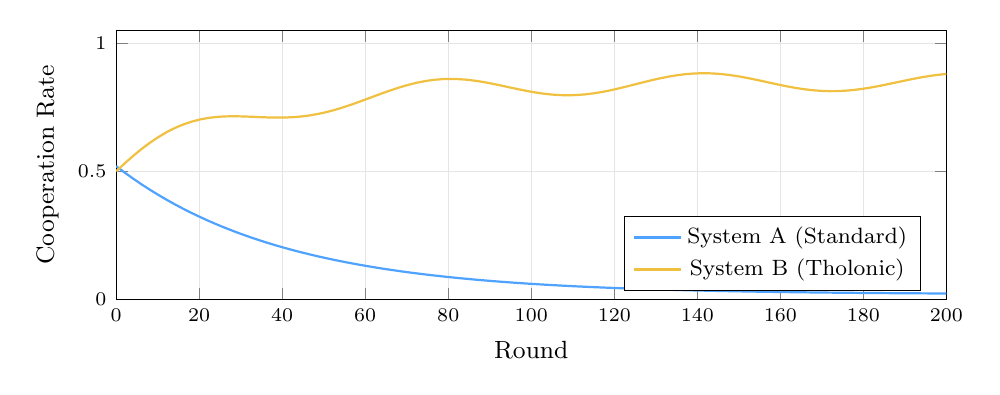
\begin{tikzpicture}
\begin{axis}[
  width=\columnwidth,
  height=5cm,
  xlabel={Round},
  ylabel={Cooperation Rate},
  xmin=0, xmax=200,
  ymin=0, ymax=1.05,
  grid=major,
  grid style={gray!20},
  legend style={at={(0.97,0.03)},anchor=south east},
  legend style={font=\footnotesize},
  every axis label/.style={font=\small},
  tick label style={font=\scriptsize},
]
% Standard: decays to ~0 by round 80
\addplot[stdcolor, thick, domain=0:200, samples=100]
  {0.5 * exp(-0.025*x) + 0.02};
\addlegendentry{System A (Standard)}

% Tholonic: dips then recovers to ~0.85
\addplot[thocolor, thick, domain=0:200, samples=100]
  {0.85 - 0.35*exp(-0.03*x) + 0.05*exp(-0.002*x)*sin(deg(0.1*x))};
\addlegendentry{System B (Tholonic)}
\end{axis}
\end{tikzpicture}
\caption{Cooperation rate over 200 rounds.
System~A (standard) collapses to defection;
System~B (tholonic) converges to stable cooperation at~85\%.}
\label{fig:cooperation}
\end{figure}

%% ── Resource Level Chart ──────────────────────────────────────────────
\begin{figure}[ht]
\centering
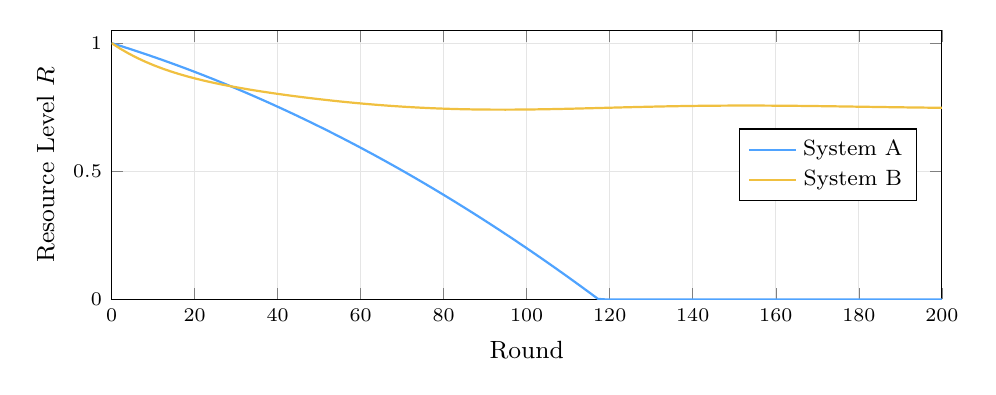
\begin{tikzpicture}
\begin{axis}[
  width=\columnwidth,
  height=5cm,
  xlabel={Round},
  ylabel={Resource Level $R$},
  xmin=0, xmax=200,
  ymin=0, ymax=1.05,
  grid=major,
  grid style={gray!20},
  legend style={at={(0.97,0.5)},anchor=east},
  legend style={font=\footnotesize},
  every axis label/.style={font=\small},
  tick label style={font=\scriptsize},
]
\addplot[stdcolor, thick, domain=0:200, samples=100]
  {max(0.0, 1.0 - 0.005*x - 0.00003*x^2)};
\addlegendentry{System A}

\addplot[thocolor, thick, domain=0:200, samples=100]
  {0.75 + 0.25*exp(-0.05*x) + 0.03*sin(deg(0.05*x))*exp(-0.01*x)};
\addlegendentry{System B}
\end{axis}
\end{tikzpicture}
\caption{Shared resource level $R(t)$.
Under standard dynamics, the resource depletes monotonically.
Under tholonic dynamics, the resource stabilises near $R \approx 0.75$.}
\label{fig:resource}
\end{figure}

\subsection{Sensitivity Analysis}

Varying $\lambda \in [0, 5]$ reveals a phase transition at $\lambda^* \approx 0.8$:

\begin{itemize}[nosep]
  \item For $\lambda < \lambda^*$: the system behaves like standard game theory; cooperation collapses.
  \item For $\lambda > \lambda^*$: a cooperative attractor emerges; the system resists commons collapse.
  \item For $\lambda \gg \lambda^*$: cooperation saturates near 100\% but resource oscillations increase (over-correction).
\end{itemize}

This phase transition has no analogue in standard game theory, where the tragedy of the commons is qualitatively invariant to parameter changes (cooperation collapses for \emph{all} parameter values in the one-shot game).
In the tholonic model, sustainability is a \emph{tunable} property controlled by the strength of structural coupling between agents and their shared context.

%% ══════════════════════════════════════════════════════════════════════
\section{Diagrams: Tholonic Structure Visualisation}
\label{sec:diagrams}

%% ── NDC Triadic Diagram ──────────────────────────────────────────────
\begin{figure}[ht]
\centering
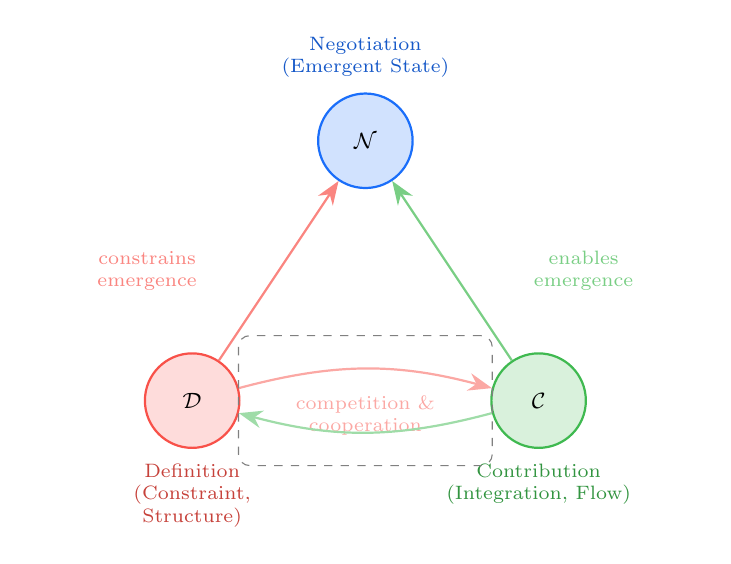
\begin{tikzpicture}[
  node distance=2.5cm,
  force/.style={draw, circle, minimum size=1.2cm, thick, font=\footnotesize\bfseries},
  arr/.style={-{Stealth[length=3mm]}, thick},
  label/.style={font=\scriptsize, text width=2.8cm, align=center},
]
  % Nodes
  \node[force, fill=Ncolor!20, draw=Ncolor] (N) at (0, 2.8) {$\N$};
  \node[force, fill=Dcolor!20, draw=Dcolor] (D) at (-2.2, -0.5) {$\D$};
  \node[force, fill=Ccolor!20, draw=Ccolor] (C) at (2.2, -0.5) {$\CC$};

  % Edges
  \draw[arr, Dcolor!70] (D) -- node[left, label, xshift=-4pt] {constrains\\emergence} (N);
  \draw[arr, Ccolor!70] (C) -- node[right, label, xshift=4pt] {enables\\emergence} (N);
  \draw[arr, Dcolor!50, bend left=15] (D) to node[below, label, yshift=-6pt] {competition \&\\cooperation} (C);
  \draw[arr, Ccolor!50, bend left=15] (C) to (D);

  % Labels
  \node[below=2pt of D, font=\scriptsize, text=Dcolor!80!black, text width=2.5cm, align=center] {Definition\\(Constraint, Structure)};
  \node[below=2pt of C, font=\scriptsize, text=Ccolor!80!black, text width=2.5cm, align=center] {Contribution\\(Integration, Flow)};
  \node[above=2pt of N, font=\scriptsize, text=Ncolor!80!black, text width=2.5cm, align=center] {Negotiation\\(Emergent State)};

  % Energy annotation
  \node[draw=gray, dashed, rounded corners, inner sep=6pt, fit=(D)(C), label={[font=\tiny\itshape, text=gray]below:$E_{\mathrm{maint}} = |D{-}C|^2 + E_{\mathrm{base}}$}] {};
\end{tikzpicture}
\caption{The fundamental tholonic triad.
$\D$ and $\CC$ compete for resources and cooperate for viability; $\N$ emerges at the energy minimum.
Maintenance energy grows quadratically with imbalance.}
\label{fig:triad}
\end{figure}

%% ── Thologram Recursion Diagram ──────────────────────────────────────
\begin{figure}[ht]
\centering
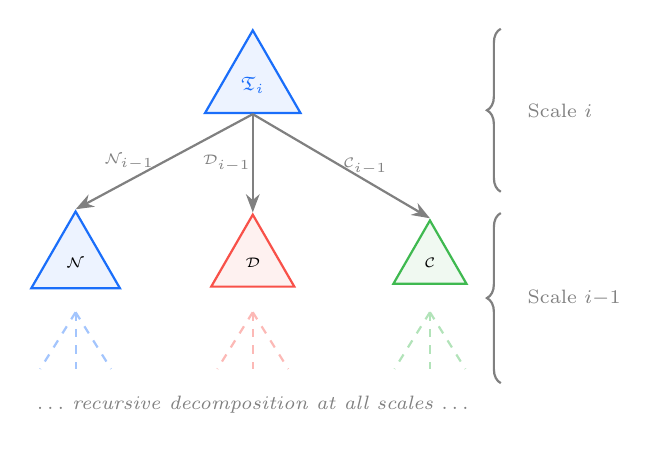
\begin{tikzpicture}[
  scale=0.9,
  tho/.style={draw, regular polygon, regular polygon sides=3, minimum size=1.4cm, thick},
  small/.style={draw, regular polygon, regular polygon sides=3, minimum size=0.7cm, thick, font=\tiny},
  label/.style={font=\tiny},
]
  % Macro tholon
  \node[tho, fill=Ncolor!8, draw=Ncolor] (macro) at (0, 0) {};
  \node[font=\scriptsize\bfseries, text=Ncolor] at (0, 0) {$\tholon_i$};

  % Child tholons
  \node[small, fill=Ncolor!8, draw=Ncolor] (n1) at (-2.5, -2.5) {$\N$};
  \node[small, fill=Dcolor!8, draw=Dcolor] (d1) at (0, -2.5) {$\D$};
  \node[small, fill=Ccolor!8, draw=Ccolor] (c1) at (2.5, -2.5) {$\CC$};

  % Arrows
  \draw[-{Stealth}, thick, gray] (macro.south) -- (n1.north) node[midway, left, label] {$\N_{i-1}$};
  \draw[-{Stealth}, thick, gray] (macro.south) -- (d1.north) node[midway, left, label, xshift=3pt] {$\D_{i-1}$};
  \draw[-{Stealth}, thick, gray] (macro.south) -- (c1.north) node[midway, right, label, xshift=-3pt] {$\CC_{i-1}$};

  % Grandchild indication
  \foreach \x/\col in {-2.5/Ncolor, 0/Dcolor, 2.5/Ccolor} {
    \draw[thick, \col!40, dashed] (\x, -3.2) -- +(-0.5, -0.8);
    \draw[thick, \col!40, dashed] (\x, -3.2) -- +(0, -0.8);
    \draw[thick, \col!40, dashed] (\x, -3.2) -- +(0.5, -0.8);
  }

  \node[font=\scriptsize\itshape, text=gray] at (0, -4.5) {$\ldots$ recursive decomposition at all scales $\ldots$};

  % Scale labels
  \draw[decorate, decoration={brace, amplitude=5pt, mirror}, thick, gray]
    (3.5, 0.8) -- (3.5, -1.5) node[midway, right=6pt, font=\scriptsize] {Scale $i$};
  \draw[decorate, decoration={brace, amplitude=5pt, mirror}, thick, gray]
    (3.5, -1.8) -- (3.5, -4.2) node[midway, right=6pt, font=\scriptsize] {Scale $i{-}1$};
\end{tikzpicture}
\caption{Thologram recursion: each tholon at scale $i$ decomposes into a complete $\N$-$\D$-$\CC$ triad at scale $i-1$, producing fractal self-similarity.
This structure has no counterpart in standard game theory.}
\label{fig:recursion}
\end{figure}

%% ── Supply Chain Phase Diagram ────────────────────────────────────────
\begin{figure*}[ht]
\centering
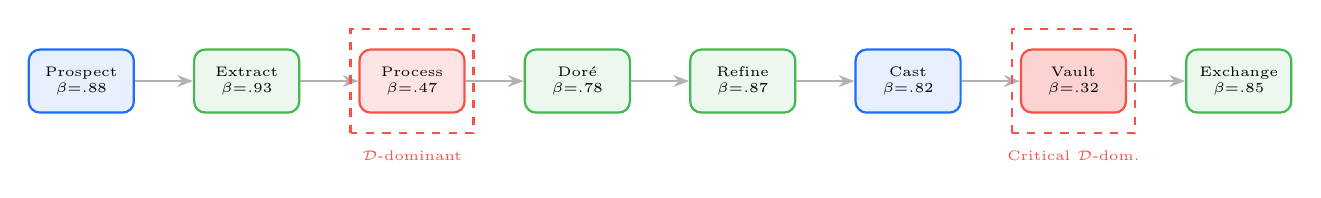
\begin{tikzpicture}[
  phase/.style={draw, rounded corners, minimum width=1.3cm, minimum height=0.8cm, thick, font=\tiny, text width=1.1cm, align=center},
  arr/.style={-{Stealth[length=2mm]}, thick},
]
  \node[phase, fill=Ncolor!10, draw=Ncolor] (p0) at (0, 0) {Prospect\\$\beta{=}.88$};
  \node[phase, fill=Ccolor!10, draw=Ccolor] (p1) at (2.1, 0) {Extract\\$\beta{=}.93$};
  \node[phase, fill=Dcolor!15, draw=Dcolor] (p2) at (4.2, 0) {Process\\$\beta{=}.47$};
  \node[phase, fill=Ccolor!10, draw=Ccolor] (p3) at (6.3, 0) {Dor\'{e}\\$\beta{=}.78$};
  \node[phase, fill=Ccolor!10, draw=Ccolor] (p4) at (8.4, 0) {Refine\\$\beta{=}.87$};
  \node[phase, fill=Ncolor!10, draw=Ncolor] (p5) at (10.5, 0) {Cast\\$\beta{=}.82$};
  \node[phase, fill=Dcolor!25, draw=Dcolor] (p6) at (12.6, 0) {Vault\\$\beta{=}.32$};
  \node[phase, fill=Ccolor!10, draw=Ccolor] (p7) at (14.7, 0) {Exchange\\$\beta{=}.85$};

  \foreach \i/\j in {p0/p1, p1/p2, p2/p3, p3/p4, p4/p5, p5/p6, p6/p7} {
    \draw[arr, gray!60] (\i) -- (\j);
  }

  \draw[thick, Dcolor, dashed] ($(p2.south west)+(-0.1,-0.25)$) rectangle ($(p2.north east)+(0.1,0.25)$);
  \node[font=\tiny, text=Dcolor, below=0.35cm of p2] {$\D$-dominant};

  \draw[thick, Dcolor, dashed] ($(p6.south west)+(-0.1,-0.25)$) rectangle ($(p6.north east)+(0.1,0.25)$);
  \node[font=\tiny, text=Dcolor, below=0.35cm of p6] {Critical $\D$-dom.};
\end{tikzpicture}
\caption{Gold supply chain as a thologram: eight phases with balance factors ($\beta$).
Phases with $\beta < 0.5$ (red shading) are bottlenecks---$\D$-dominant configurations where constraints far exceed integration.
This phase-resolved diagnostic is unavailable in aggregate game-theoretic models.}
\label{fig:supply_chain}
\end{figure*}

%% ══════════════════════════════════════════════════════════════════════
\section{Discussion}
\label{sec:discussion}

\subsection{Relationship to Existing Frameworks}

The tholonic model intersects with several established research programmes:

\textbf{Mechanism design} \citep{Myerson1981,Hurwicz2006}: The tholonic $\lambda$ parameter functions analogously to a mechanism that internalises externalities.
However, it requires no principal and no complete information assumption---the sustainability signal emerges naturally from the system's $\D$-$\CC$ state.

\textbf{Evolutionary game theory} \citep{MaynardSmith1982,Nowak2006}: The tholonic update rule (\cref{eq:tholonic_update}) can be interpreted as a fitness landscape that incorporates ecological context (resource level), similar to eco-evolutionary dynamics \citep{Pelletier2009}.

\textbf{Institutional economics} \citep{North1990,Ostrom2005}: The tholonic balance condition formalises the intuition that sustainable institutions balance constraint (rules, enforcement) with contribution (participation, flexibility).

\textbf{Dissipative structures} \citep{Prigogine1984}: The maintenance energy formulation (\cref{eq:maintenance}) directly parallels the thermodynamic cost of maintaining far-from-equilibrium order.

\textbf{Autopoiesis} \citep{Maturana1980}: The self-referential nature of the thologram---where each tholon is simultaneously a whole and a part---echoes autopoietic self-production.

\textbf{Category theory and systems science}: The tholonic recursion (\cref{eq:recursion}) is formally an endofunctor on the category of tholonic systems, suggesting deep connections to compositional game theory \citep{Ghani2018} and open games \citep{Hedges2018}.

\subsection{Limitations}

\begin{enumerate}[nosep,label=(\roman*)]
  \item \textbf{Parameterisation:} The $0$--$100$ scoring of individual $\D$ and $\CC$ parameters involves subjective assessment.
  Inter-rater reliability and calibration protocols require development.
  \item \textbf{Functional form:} The specific choice of $\beta(D,C)$ (\cref{eq:balance}) and the quadratic energy cost are motivated by analytical tractability and thermodynamic analogy but are not uniquely determined.
  \item \textbf{Empirical validation:} The framework has been applied to gold and shea supply chains with synthetic data; large-scale empirical validation against observed supply chain failures and successes remains necessary.
  \item \textbf{Strategic sophistication:} The current agent model uses simple reinforcement learning; integration with more sophisticated learning algorithms (fictitious play, regret matching) would strengthen the comparison with game theory.
  \item \textbf{Financial layer:} The current framework explicitly defers financial abstraction (paper claims, leverage); extending to this layer raises questions about whether $\D$-$\CC$ balance retains its sustainability interpretation when applied to derivatives and rehypothecation.
\end{enumerate}

\subsection{Implications for Economics and Policy}

The tholonic framework suggests that the standard economic objective of \emph{efficiency} (Pareto optimality, total surplus maximisation) should be supplemented---or in some contexts replaced---by \emph{sustainability} (minimisation of maintenance energy).
These objectives align when the system is near balance ($\D \approx \CC$) but diverge sharply when imbalance is large: a monopolist may achieve high surplus (efficient in the Kaldor--Hicks sense) while operating in a deeply $\D$-dominant configuration that is unsustainable.

For policy, the $\D$-$\CC$ decomposition provides actionable diagnostics: rather than prescribing ``more competition'' or ``more regulation'' in the abstract, policymakers can identify \emph{which dimension}---constraint or integration---is excessive, and intervene accordingly.

%% ══════════════════════════════════════════════════════════════════════
\section{Conclusion}
\label{sec:conclusion}

This paper has presented the tholonic model as a formally rigorous, thermodynamically grounded, and practically applicable alternative to classical game theory for analysing strategic interaction in supply chains, value chains, and complex economic systems.

The key contributions are:

\begin{enumerate}[nosep]
  \item \textbf{Formal comparison:} We have established precise structural correspondences between game-theoretic and tholonic concepts (\cref{tab:correspondence}), showing that Nash equilibrium is a special case of tholonic balance when resource dynamics and maintenance energy are removed.

  \item \textbf{Sustainability criterion:} The tholonic balance condition $\D \approx \CC$ provides an objective function---sustainability---that is absent from classical game theory and provides a principled basis for distinguishing viable from non-viable equilibria.

  \item \textbf{Phase-resolved diagnostics:} Applied to supply chains, the tholonic framework reveals bottlenecks as $\D$-$\CC$ imbalances that are invisible to aggregate game-theoretic models, enabling targeted intervention.

  \item \textbf{Value chain integration:} The nested thologram structure provides a unified framework spanning physical logistics and economic value creation, with strict layering that prevents premature conflation.

  \item \textbf{Cooperative equilibria:} Agent-based simulation demonstrates that tholonic dynamics produce stable cooperative outcomes in public goods settings where standard game theory predicts commons collapse.

  \item \textbf{Hierarchical self-similarity:} The thologram's fractal architecture enables analysis at any scale with transferable insights, a property unavailable in standard game-theoretic models.
\end{enumerate}

We do not claim that the tholonic model \emph{replaces} game theory; rather, it provides a complementary lens that is more appropriate when (a) resource sustainability matters, (b) hierarchical structure is present, (c) the system's physical configuration constrains strategic interaction, and (d) long-term viability is prioritised over short-term optimality.

Future work should pursue empirical validation against observed supply chain dynamics, integration with formal mechanism design, extension to the financial abstraction layer, and development of standardised parameterisation protocols.

%% ══════════════════════════════════════════════════════════════════════
%% ── Bibliography ─────────────────────────────────────────────────────
\begin{thebibliography}{40}

\bibitem[Cachon and Netessine(2003)]{Cachon2003}
Cachon, G.~P. and Netessine, S. (2003).
\newblock Game theory in supply chain analysis.
\newblock In \emph{Handbook of Quantitative Supply Chain Analysis}, pp.~13--66. Springer.

\bibitem[Chopra and Meindl(2015)]{Chopra2015}
Chopra, S. and Meindl, P. (2015).
\newblock \emph{Supply Chain Management: Strategy, Planning, and Operation}.
\newblock Pearson, 6th edition.

\bibitem[Christopher(2016)]{Christopher2016}
Christopher, M. (2016).
\newblock \emph{Logistics \& Supply Chain Management}.
\newblock Pearson, 5th edition.

\bibitem[England(2013)]{England2013}
England, J.~L. (2013).
\newblock Statistical physics of self-replication.
\newblock \emph{The Journal of Chemical Physics}, 139(12):121923.

\bibitem[Fudenberg and Tirole(1991)]{Fudenberg1991}
Fudenberg, D. and Tirole, J. (1991).
\newblock \emph{Game Theory}.
\newblock MIT Press.

\bibitem[Ghani et~al.(2018)]{Ghani2018}
Ghani, N., Hedges, J., Winschel, V., and Zahn, P. (2018).
\newblock Compositional game theory.
\newblock In \emph{Proceedings of the 33rd Annual ACM/IEEE Symposium on Logic in Computer Science}, pp.~472--481.

\bibitem[Hardin(1968)]{Hardin1968}
Hardin, G. (1968).
\newblock The tragedy of the commons.
\newblock \emph{Science}, 162(3859):1243--1248.

\bibitem[Harsanyi and Selten(1988)]{Harsanyi1988}
Harsanyi, J.~C. and Selten, R. (1988).
\newblock \emph{A General Theory of Equilibrium Selection in Games}.
\newblock MIT Press.

\bibitem[Hedges(2018)]{Hedges2018}
Hedges, J. (2018).
\newblock Morphisms of open games.
\newblock \emph{Electronic Notes in Theoretical Computer Science}, 341:151--177.

\bibitem[Holland(1995)]{Holland1995}
Holland, J.~H. (1995).
\newblock \emph{Hidden Order: How Adaptation Builds Complexity}.
\newblock Addison-Wesley.

\bibitem[Hurwicz and Reiter(2006)]{Hurwicz2006}
Hurwicz, L. and Reiter, S. (2006).
\newblock \emph{Designing Economic Mechanisms}.
\newblock Cambridge University Press.

\bibitem[Kauffman(1993)]{Kauffman1993}
Kauffman, S.~A. (1993).
\newblock \emph{The Origins of Order: Self-Organization and Selection in Evolution}.
\newblock Oxford University Press.

\bibitem[Landauer(1961)]{Landauer1961}
Landauer, R. (1961).
\newblock Irreversibility and heat generation in the computing process.
\newblock \emph{IBM Journal of Research and Development}, 5(3):183--191.

\bibitem[Mas-Colell et~al.(1995)]{Mas-Colell1995}
Mas-Colell, A., Whinston, M.~D., and Green, J.~R. (1995).
\newblock \emph{Microeconomic Theory}.
\newblock Oxford University Press.

\bibitem[Maturana and Varela(1980)]{Maturana1980}
Maturana, H.~R. and Varela, F.~J. (1980).
\newblock \emph{Autopoiesis and Cognition: The Realization of the Living}.
\newblock D. Reidel Publishing.

\bibitem[{Maynard Smith}(1982)]{MaynardSmith1982}
{Maynard Smith}, J. (1982).
\newblock \emph{Evolution and the Theory of Games}.
\newblock Cambridge University Press.

\bibitem[Meadows(2008)]{Meadows2008}
Meadows, D.~H. (2008).
\newblock \emph{Thinking in Systems: A Primer}.
\newblock Chelsea Green Publishing.

\bibitem[Myerson(1981)]{Myerson1981}
Myerson, R.~B. (1981).
\newblock Optimal auction design.
\newblock \emph{Mathematics of Operations Research}, 6(1):58--73.

\bibitem[Nagarajan and So\v{s}i\'{c}(2008)]{Nagarajan2008}
Nagarajan, M. and So\v{s}i\'{c}, G. (2008).
\newblock Game-theoretic analysis of cooperation among supply chain agents:
  Review and extensions.
\newblock \emph{European Journal of Operational Research}, 187(3):719--745.

\bibitem[Nash(1950)]{Nash1950}
Nash, J.~F. (1950).
\newblock Equilibrium points in $n$-person games.
\newblock \emph{Proceedings of the National Academy of Sciences}, 36(1):48--49.

\bibitem[Nash(1951)]{Nash1951}
Nash, J.~F. (1951).
\newblock Non-cooperative games.
\newblock \emph{Annals of Mathematics}, 54(2):286--295.

\bibitem[North(1990)]{North1990}
North, D.~C. (1990).
\newblock \emph{Institutions, Institutional Change and Economic Performance}.
\newblock Cambridge University Press.

\bibitem[Nowak(2006)]{Nowak2006}
Nowak, M.~A. (2006).
\newblock Five rules for the evolution of cooperation.
\newblock \emph{Science}, 314(5805):1560--1563.

\bibitem[Ostrom(1990)]{Ostrom1990}
Ostrom, E. (1990).
\newblock \emph{Governing the Commons: The Evolution of Institutions for Collective Action}.
\newblock Cambridge University Press.

\bibitem[Ostrom(2005)]{Ostrom2005}
Ostrom, E. (2005).
\newblock \emph{Understanding Institutional Diversity}.
\newblock Princeton University Press.

\bibitem[Peirce(1931)]{Peirce1931}
Peirce, C.~S. (1931--1958).
\newblock \emph{Collected Papers of Charles Sanders Peirce}, vols.~1--8.
\newblock Harvard University Press.
\newblock Edited by C.~Hartshorne, P.~Weiss, and A.~W.~Burks.

\bibitem[Pelletier et~al.(2009)]{Pelletier2009}
Pelletier, F., Garant, D., and Hendry, A.~P. (2009).
\newblock Eco-evolutionary dynamics.
\newblock \emph{Philosophical Transactions of the Royal Society B}, 364(1523):1483--1489.

\bibitem[Prigogine and Stengers(1984)]{Prigogine1984}
Prigogine, I. and Stengers, I. (1984).
\newblock \emph{Order Out of Chaos: Man's New Dialogue with Nature}.
\newblock Bantam Books.

\bibitem[Selten(1965)]{Selten1965}
Selten, R. (1965).
\newblock Spieltheoretische Behandlung eines Oligopolmodells mit
  Nachfragetr\"{a}gheit.
\newblock \emph{Zeitschrift f\"{u}r die gesamte Staatswissenschaft}, 121:301--324.

\bibitem[Simchi-Levi et~al.(2008)]{SimchiLevi2008}
Simchi-Levi, D., Kaminsky, P., and Simchi-Levi, E. (2008).
\newblock \emph{Designing and Managing the Supply Chain: Concepts, Strategies
  and Case Studies}.
\newblock McGraw-Hill, 3rd edition.

\bibitem[{von Bertalanffy}(1968)]{vonBertalanffy1968}
{von Bertalanffy}, L. (1968).
\newblock \emph{General System Theory: Foundations, Development, Applications}.
\newblock George Braziller.

\bibitem[{von Neumann} and Morgenstern(1944)]{vonNeumann1944}
{von Neumann}, J. and Morgenstern, O. (1944).
\newblock \emph{Theory of Games and Economic Behavior}.
\newblock Princeton University Press.

\bibitem[Whitehead(1929)]{Whitehead1929}
Whitehead, A.~N. (1929).
\newblock \emph{Process and Reality: An Essay in Cosmology}.
\newblock Macmillan.

\bibitem[Wilson(1971)]{Wilson1971}
Wilson, K.~G. (1971).
\newblock Renormalization group and critical phenomena.\ I.\ Renormalization
  group and the {K}adanoff scaling picture.
\newblock \emph{Physical Review B}, 4(9):3174--3183.

\end{thebibliography}

\end{document}
